% effective_sources.tex — Multipole Effective Sources and Dependent Field Jumps
% Compile with: lualatex effective_sources.tex
\documentclass[11pt,a4paper]{article}

\usepackage{fontspec}
\setmainfont{Latin Modern Roman}
\setmonofont{Latin Modern Mono}

\usepackage{amsmath,amssymb,amsthm}
\usepackage{mathtools}
\usepackage{bm}
\usepackage{booktabs}
\usepackage[svgnames]{xcolor}
\usepackage{geometry}
\geometry{margin=2.5cm}

\usepackage{hyperref}
\hypersetup{
  colorlinks=true,
  linkcolor=DarkBlue,
  citecolor=DarkBlue,
  urlcolor=DarkBlue,
}

\usepackage{enumitem}
\usepackage{fancyhdr}
\pagestyle{fancy}
\fancyhf{}
\fancyhead[L]{\small Multipole Effective Sources in the 9$\times$9 Displacement-Strain Basis}
\fancyhead[R]{\small\thepage}
\renewcommand{\headrulewidth}{0.4pt}

% TikZ
\usepackage{tikz}
\usetikzlibrary{arrows.meta,positioning,shapes.geometric,patterns,calc,decorations.pathmorphing}

% Notation shortcuts
\newcommand{\dd}{\mathrm{d}}
\newcommand{\eps}{\varepsilon}
\newcommand{\rrn}{\bm{r}_n}
\newcommand{\nn}{\hat{\bm{n}}}
\newcommand{\uu}{\bm{u}}
\newcommand{\tr}{\operatorname{tr}}
\newcommand{\dev}{\mathrm{dev}}
\newcommand{\jump}[1]{\left[\kern-1.5pt\left[#1\right]\kern-1.5pt\right]}

\theoremstyle{plain}
\newtheorem{proposition}{Proposition}
\newtheorem{lemma}[proposition]{Lemma}
\newtheorem{theorem}[proposition]{Theorem}
\theoremstyle{definition}
\newtheorem{definition}[proposition]{Definition}
\theoremstyle{remark}
\newtheorem{remark}[proposition]{Remark}

\title{%
  Multipole Effective Sources and Dependent Field Jumps\\
  in the $9{\times}9$ Displacement-Strain Basis for Elastic Scattering%
}
\author{}
\date{}

\begin{document}
\maketitle
\thispagestyle{fancy}

\begin{abstract}
We analyse how the contrast of a small elastic inclusion in a homogeneous
background radiates as a superposition of effective multipole sources, and
show how those sources manifest as discontinuities in the \emph{dependent}
components of the displacement--strain field.  Working in the coupled
nine-component basis $\psi = (u_i,\eps_{jk})$ used by Foldy--Lax multiple
scattering solvers, we identify the $\mathrm{SO}(3)$ irreducible
decomposition of $\psi$ into a monopole (trace strain $\eps_{kk}$,
$\ell=0$), a dipole (displacement $\bm{u}$, $\ell=1$), and a quadrupole
(deviatoric strain $\eps_{ij}^{\dev}$, $\ell=2$), with multiplicities
$1+3+5=9$.  The three components $\eps_{zz}$, $\eps_{xz}$, $\eps_{yz}$
involving a normal derivative across a material interface are the
\emph{dependent} ones: we derive the closed-form jump conditions for these
components from continuity of displacement and traction, and show that the
resulting jumps are sourced respectively by a density contrast
(dipole/body-force channel), a bulk-modulus contrast (monopole/explosion
channel) and a shear-modulus contrast (quadrupole/deviatoric channel).
An elementary parity argument shows that the corresponding local
$T$-matrix is block-diagonal between the $\ell=1$ (dipole) sector and the
$(\ell=0)\oplus(\ell=2)$ (monopole/quadrupole) sector at leading order in
the inclusion size, and that the $9\times 9$ basis is
\emph{minimal} for representing all three contrast channels in a single
self-contained Lippmann--Schwinger framework.
\end{abstract}

\tableofcontents
\vspace{0.5em}

%=============================================================================
\section{Introduction}\label{sec:intro}
%=============================================================================
Multiple scattering of elastic waves from small heterogeneities is
classically formulated as a Lippmann--Schwinger equation with a
frequency-domain Green's operator and a local scattering operator
(a ``$T$-matrix'') that encapsulates everything about the
inclusion~\cite{foldy1945,martin2006}.  The choice of the state vector
$\psi$ on which the Green's operator acts is not arbitrary: it must be
rich enough to carry all degrees of freedom that couple to the
material contrasts, and small enough that the solver is numerically
tractable.

For an inclusion with three independent Lam\'e contrasts
$(\Delta\lambda,\Delta\mu,\Delta\rho)$ embedded in an isotropic elastic
background, the natural choice is the nine-component
displacement--strain vector
\begin{equation}
  \psi
  \;=\;
  (u_1,u_2,u_3,\;\eps_{11},\eps_{22},\eps_{33},
         \eps_{23},\eps_{13},\eps_{12}),
  \label{eq:psi-nine}
\end{equation}
in which all three contrasts act as multiplicative operators with no
derivatives at the inclusion.  Six of these nine components --- the three
displacements $u_i$ and the three in-plane strains
$\eps_{xx},\eps_{yy},\eps_{xy}$ --- are \emph{continuous} across a
material interface aligned with the horizontal plane; the remaining
three, $\eps_{zz}$, $\eps_{xz}$, $\eps_{yz}$, carry a normal derivative
$\partial_z u_k$ and are \emph{dependent}: they jump discontinuously
across the interface whenever the Lam\'e parameters do.

\begin{quote}
\textit{The purpose of this note is to show that these three jumps are
not a nuisance but a physically lucid statement of the multipole
structure of the effective source.}  Density contrast drives the
\emph{dipole} (body-force) channel, bulk-modulus contrast drives the
\emph{monopole} (explosion) channel, and shear-modulus contrast drives
the \emph{quadrupole} (double-couple) channel.  The three dependent
components are exactly those on which these three multipoles write their
signatures, with the dependence dictated by the $\mathrm{SO}(3)$
representation theory of the strain tensor.
\end{quote}

\medskip
\noindent
The paper is organised as follows.  In Section~\ref{sec:basis} we set
out the nine-component basis and record the isotropic constitutive law.
Section~\ref{sec:irrep} carries out the $\mathrm{SO}(3)$ irreducible
decomposition of $\psi$ into monopole, dipole and quadrupole pieces.
Section~\ref{sec:jumps} derives the jump conditions across a horizontal
material interface and identifies the three dependent components.
Section~\ref{sec:sources} assembles the effective source density in the
first Born approximation and reads off the assignment
$\Delta\rho\mapsto\text{dipole}$, $\Delta\kappa\mapsto\text{monopole}$,
$\Delta\mu\mapsto\text{quadrupole}$.  Section~\ref{sec:tblock} shows
that the local $T$-matrix is block-diagonal in the parity-even versus
parity-odd sectors, and Section~\ref{sec:minimality} states and proves
a minimality theorem for the basis~\eqref{eq:psi-nine}.
Section~\ref{sec:conclusions} concludes.

%=============================================================================
\section{The Nine-Component Basis}\label{sec:basis}
%=============================================================================
Let $(\uu,\bm{\eps})$ denote the displacement field $u_i(\bm{r})$ and
the infinitesimal strain tensor
$\eps_{ij}=\tfrac{1}{2}(\partial_i u_j+\partial_j u_i)$ in an isotropic
elastic background with Lam\'e parameters $(\lambda,\mu)$, density
$\rho$, and time-harmonic dependence $e^{-i\omega t}$.  The stress
tensor obeys Hooke's law,
\begin{equation}
  \sigma_{ij}
  \;=\;
  \lambda\,\eps_{kk}\,\delta_{ij} + 2\mu\,\eps_{ij},
  \label{eq:hooke}
\end{equation}
and the frequency-domain momentum balance reads
\begin{equation}
  \partial_j\sigma_{ij} + \rho\omega^2 u_i \;=\; -f_i,
  \label{eq:momentum}
\end{equation}
with $f_i$ an external body force.  We gather the nine scalar fields
into the column vector $\psi = (u_i,\eps_{jk})^\top\in\mathbb{C}^9$
defined in~\eqref{eq:psi-nine}, ordering the strain block by the six
independent symmetric components
$(\eps_{11},\eps_{22},\eps_{33},\eps_{23},\eps_{13},\eps_{12})$.

Although six strain components appear kinematically redundant given three
displacements, they are \emph{not} redundant dynamically, because the
Lam\'e contrasts $(\Delta\lambda,\Delta\mu)$ couple to specific linear
combinations of the strain.  Carrying the full strain tensor in the
state vector allows the local scattering operator to act on
$\psi(\rrn)$ by pointwise matrix multiplication, with no spatial
derivatives entering the scatterer itself --- the derivatives are
absorbed into the Green's operator that links scatterers.

\begin{remark}
The strain $\eps_{ij}$ appears in $\psi$ as an \emph{independent} datum
from $\uu$, even though it is algebraically a derivative of $\uu$.  The
solver treats~\eqref{eq:psi-nine} as nine unknowns linked by the
Green's operator, whose consistency is only imposed at the scatterer
positions.  This is the standard Lippmann--Schwinger
reformulation of elastodynamics~\cite{martin2006,kennett2001}.
\end{remark}

%=============================================================================
\section{Irreducible Decomposition Under Rotations}\label{sec:irrep}
%=============================================================================
Under the rotation group $\mathrm{SO}(3)$, $\uu$ transforms as a vector
(spin $\ell=1$), while the symmetric strain tensor $\eps_{ij}$
decomposes uniquely into its trace and deviator,
\begin{equation}
  \eps_{ij}
  \;=\;
  \underbrace{\tfrac{1}{3}\,\eps_{kk}\,\delta_{ij}}_{\ell=0\;(\text{scalar})}
  \;+\;
  \underbrace{\eps_{ij}^{\dev}}_{\ell=2\;(\text{symmetric traceless})},
  \qquad
  \eps_{ij}^{\dev}\delta_{ij}=0,
  \label{eq:strain-split}
\end{equation}
carrying $\ell=0$ and $\ell=2$ irreducible representations with
multiplicities $1$ and $5$ respectively.  Together with the $\ell=1$
displacement, the nine-component basis decomposes as
\begin{equation}
  \psi \;\in\;
  \underbrace{\mathbf{1}}_{\substack{\ell=0\\ \text{monopole}}}
  \;\oplus\;
  \underbrace{\mathbf{3}}_{\substack{\ell=1\\ \text{dipole}}}
  \;\oplus\;
  \underbrace{\mathbf{5}}_{\substack{\ell=2\\ \text{quadrupole}}},
  \qquad
  1 + 3 + 5 \;=\; 9,
  \label{eq:irrep-sum}
\end{equation}
with multiplicities summing to the $9$ components of~$\psi$.

Figure~\ref{fig:decomposition} sketches the decomposition.  Reading the
tree physically: the trace strain $\eps_{kk}$ represents isotropic
compression/expansion and radiates as an \emph{explosion} monopole; the
displacement vector $\uu$ transforms as a body-force \emph{dipole}; the
deviatoric strain $\eps_{ij}^{\dev}$ carries the five independent
shear-distortion modes and radiates as a symmetric-traceless
\emph{quadrupole} (``double couple'').

\begin{figure}[t]
\centering
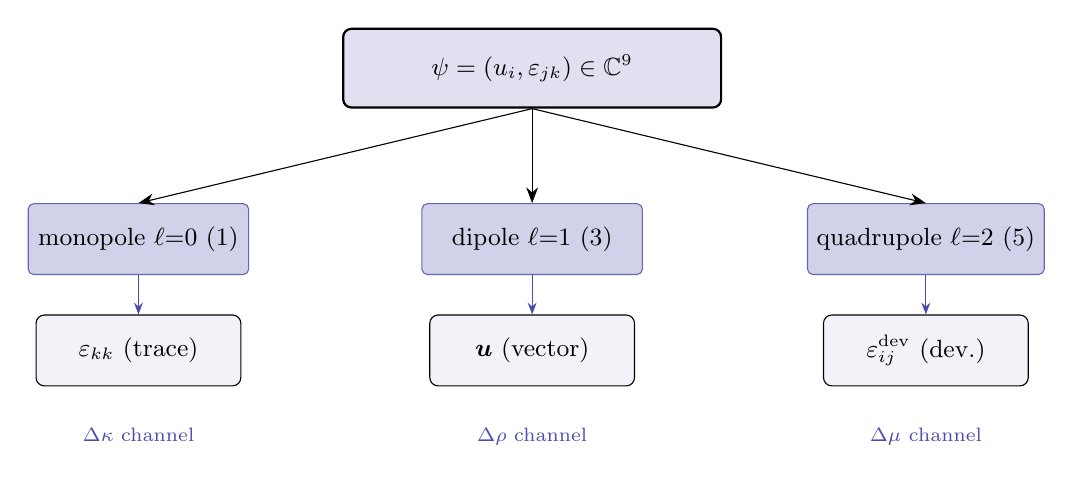
\begin{tikzpicture}[
  node distance=8mm and 16mm,
  every node/.style={font=\small},
  rep/.style={draw, rounded corners=3pt, minimum width=26mm, minimum height=9mm, fill=DarkBlue!5},
  root/.style={draw, thick, rounded corners=3pt, minimum width=48mm, minimum height=10mm, fill=DarkBlue!12},
  irr/.style={draw=DarkBlue!60, rounded corners=2pt, minimum width=28mm, minimum height=9mm, fill=DarkBlue!18},
]
  \node[root] (psi) {$\psi=(u_i,\eps_{jk})\in\mathbb{C}^9$};
  \node[irr, below=12mm of psi, xshift=-50mm] (mono) {monopole $\ell{=}0$ (1)};
  \node[irr, below=12mm of psi] (dip)  {dipole $\ell{=}1$ (3)};
  \node[irr, below=12mm of psi, xshift=50mm] (quad) {quadrupole $\ell{=}2$ (5)};

  \draw[-{Stealth[length=2mm]}] (psi.south) -- (mono.north);
  \draw[-{Stealth[length=2mm]}] (psi.south) -- (dip.north);
  \draw[-{Stealth[length=2mm]}] (psi.south) -- (quad.north);

  \node[rep, below=5mm of mono] (monoF) {$\eps_{kk}$ (trace)};
  \node[rep, below=5mm of dip]  (dipF)  {$\uu$ (vector)};
  \node[rep, below=5mm of quad] (quadF) {$\eps_{ij}^{\dev}$ (dev.)};

  \draw[-{Stealth[length=1.5mm]}, DarkBlue!70] (mono.south) -- (monoF.north);
  \draw[-{Stealth[length=1.5mm]}, DarkBlue!70] (dip.south)  -- (dipF.north);
  \draw[-{Stealth[length=1.5mm]}, DarkBlue!70] (quad.south) -- (quadF.north);

  \node[below=4mm of monoF, text=DarkBlue!70]  {\scriptsize $\Delta\kappa$ channel};
  \node[below=4mm of dipF,  text=DarkBlue!70]  {\scriptsize $\Delta\rho$ channel};
  \node[below=4mm of quadF, text=DarkBlue!70]  {\scriptsize $\Delta\mu$ channel};
\end{tikzpicture}
\caption{Irreducible decomposition of the nine-component
displacement--strain basis under $\mathrm{SO}(3)$.  The trace strain
$\eps_{kk}$ is an $\ell=0$ scalar coupling to bulk-modulus contrast
$\Delta\kappa$; the displacement $\uu$ is an $\ell=1$ vector coupling
to density contrast $\Delta\rho$; the deviatoric strain
$\eps_{ij}^{\dev}$ is the symmetric traceless $\ell=2$ tensor coupling
to shear-modulus contrast $\Delta\mu$.  The multiplicities sum to
$1+3+5=9$.}
\label{fig:decomposition}
\end{figure}

\subsection{Explicit projection operators}\label{sec:projections}

It is useful to have the projectors onto each irreducible sector in
closed form, since the solver evaluates them repeatedly on every
scatterer.  Let
\begin{equation}
  \psi \;=\; \begin{pmatrix} \uu \\ \bm{\eps} \end{pmatrix}
  \;\in\; \mathbb{C}^3\oplus \mathbb{C}^6,
  \qquad
  \bm{\eps}=(\eps_{11},\eps_{22},\eps_{33},\eps_{23},\eps_{13},\eps_{12})^\top,
  \label{eq:psi-voigt}
\end{equation}
where $\bm{\eps}$ is stored in the six-dimensional Voigt vector above,
keeping factors of unity (not two) on the off-diagonal entries so that
the inner product $\|\bm{\eps}\|^2 = \eps_{ij}\eps_{ij}$ obtains with the
standard Euclidean norm after a rescaling
\begin{equation}
  \tilde{\bm{\eps}}
  \;=\;
  (\eps_{11},\eps_{22},\eps_{33},\sqrt{2}\,\eps_{23},\sqrt{2}\,\eps_{13},\sqrt{2}\,\eps_{12})^\top.
  \label{eq:voigt-norm}
\end{equation}

\paragraph{Dipole projector ($\ell=1$).}
The displacement sector is already an $\mathrm{SO}(3)$ irreducible, so
its projector is simply the upper block identity
\begin{equation}
  P_{\ell=1}
  \;=\;
  \begin{pmatrix}
    \mathbb{I}_3 & 0_{3\times 6}\\
    0_{6\times 3} & 0_{6\times 6}
  \end{pmatrix}
  \;\in\;\mathbb{C}^{9\times 9}.
  \label{eq:P1}
\end{equation}
The projection \emph{out of} the basis is
$\pi_{\ell=1}\psi = \uu$, and the injection back is
$\iota_{\ell=1}\uu=(\uu,\bm{0})$, so that
$P_{\ell=1}=\iota_{\ell=1}\pi_{\ell=1}$.

\paragraph{Monopole projector ($\ell=0$).}
The trace strain is a scalar, and the projection from
$\bm{\eps}$ onto its $\ell=0$ subspace is
\begin{equation}
  \pi_{\ell=0}\,\bm{\eps}
  \;=\;
  \tfrac{1}{\sqrt{3}}\,(\eps_{11}+\eps_{22}+\eps_{33})
  \;\equiv\; \tfrac{1}{\sqrt{3}}\,\tr\bm{\eps}.
\end{equation}
The factor $1/\sqrt{3}$ makes the projection an isometry from the
Frobenius inner product on symmetric tensors to the Euclidean inner
product on $\mathbb{R}$.  The injection is
$\iota_{\ell=0}(m)=\tfrac{m}{\sqrt{3}}(1,1,1,0,0,0)^\top$, and the
full $9\times 9$ monopole projector is
\begin{equation}
  P_{\ell=0}
  \;=\;
  \frac{1}{3}
  \begin{pmatrix}
    0_{3\times 3} & 0_{3\times 6}\\[2pt]
    0_{6\times 3} &
    \begin{pmatrix}
      1 & 1 & 1 & 0 & 0 & 0\\
      1 & 1 & 1 & 0 & 0 & 0\\
      1 & 1 & 1 & 0 & 0 & 0\\
      0 & 0 & 0 & 0 & 0 & 0\\
      0 & 0 & 0 & 0 & 0 & 0\\
      0 & 0 & 0 & 0 & 0 & 0\\
    \end{pmatrix}
  \end{pmatrix}.
  \label{eq:P0}
\end{equation}

\paragraph{Quadrupole projector ($\ell=2$).}
The deviatoric strain sector has five real dimensions, which we take as
the orthonormal basis
\begin{equation}
  \{\,
    \mathsf{e}_{1},\,\mathsf{e}_{2},\,\mathsf{e}_{3},\,\mathsf{e}_{4},\,\mathsf{e}_{5}
  \,\},
\end{equation}
with
\begin{align}
  \mathsf{e}_{1}
  &\;=\; \tfrac{1}{\sqrt{6}}\,(2\,\hat{\bm{z}}\hat{\bm{z}}
           - \hat{\bm{x}}\hat{\bm{x}} - \hat{\bm{y}}\hat{\bm{y}})
   \;\longleftrightarrow\;
   \tfrac{1}{\sqrt{6}}(-1,-1,2,0,0,0)^\top,
  \\
  \mathsf{e}_{2}
  &\;=\; \tfrac{1}{\sqrt{2}}\,(\hat{\bm{x}}\hat{\bm{x}}-\hat{\bm{y}}\hat{\bm{y}})
   \;\longleftrightarrow\;
   \tfrac{1}{\sqrt{2}}(1,-1,0,0,0,0)^\top,
  \\
  \mathsf{e}_{3}
  &\;=\; \hat{\bm{y}}\hat{\bm{z}}+\hat{\bm{z}}\hat{\bm{y}}
   \;\longleftrightarrow\;
   (0,0,0,1,0,0)^\top,
  \\
  \mathsf{e}_{4}
  &\;=\; \hat{\bm{x}}\hat{\bm{z}}+\hat{\bm{z}}\hat{\bm{x}}
   \;\longleftrightarrow\;
   (0,0,0,0,1,0)^\top,
  \\
  \mathsf{e}_{5}
  &\;=\; \hat{\bm{x}}\hat{\bm{y}}+\hat{\bm{y}}\hat{\bm{x}}
   \;\longleftrightarrow\;
   (0,0,0,0,0,1)^\top,
\end{align}
where the right-hand expressions are the coordinates in the
$\sqrt{2}$-rescaled Voigt basis~\eqref{eq:voigt-norm}.  Collecting the
five columns into a $6\times 5$ matrix $U_{\ell=2}$, the projector onto
the deviator is
\begin{equation}
  P_{\ell=2}
  \;=\;
  \begin{pmatrix}
    0_{3\times 3} & 0_{3\times 6}\\
    0_{6\times 3} & U_{\ell=2}\,U_{\ell=2}^{\!\top}
  \end{pmatrix}
  \;=\;
  \mathbb{I}_{\bm{\eps}} \;-\; P_{\ell=0}
  \quad\text{restricted to the strain block},
  \label{eq:P2}
\end{equation}
with the second equality being the orthogonal complement statement
$\bm{\eps} = \tfrac{1}{3}(\tr\bm{\eps})\bm{1} + \bm{\eps}^{\dev}$.

\paragraph{Resolution of identity.}
The three projectors are mutually orthogonal and resolve the identity
on $\mathbb{C}^9$,
\begin{equation}
  P_{\ell=0} + P_{\ell=1} + P_{\ell=2} \;=\; \mathbb{I}_9,
  \qquad
  P_{\ell=a}P_{\ell=b} \;=\; \delta_{ab}P_{\ell=a},
  \label{eq:resolution}
\end{equation}
and their traces are the multiplicities
$\operatorname{tr}P_{\ell=0}=1$,
$\operatorname{tr}P_{\ell=1}=3$, $\operatorname{tr}P_{\ell=2}=5$.
Any state $\psi\in\mathbb{C}^9$ decomposes as
\begin{equation}
  \psi
  \;=\;
  P_{\ell=0}\psi \;+\; P_{\ell=1}\psi \;+\; P_{\ell=2}\psi,
  \label{eq:psi-decomp}
\end{equation}
with each summand living in a distinct $\mathrm{SO}(3)$ irreducible
sector.

\subsection{Projection/injection between sectors and $\mathbb{C}^9$}

It is also useful to write down the sector-level projection
and injection maps explicitly, since the solver applies them to
individual scatterers:
\begin{equation}
\begin{aligned}
  \pi_{\ell=1}&: \mathbb{C}^9 \to \mathbb{C}^3,\quad
  \pi_{\ell=1}\psi = \uu,\\
  \pi_{\ell=0}&: \mathbb{C}^9 \to \mathbb{C},\quad
  \pi_{\ell=0}\psi = \tfrac{1}{\sqrt{3}}\tr\bm{\eps},\\
  \pi_{\ell=2}&: \mathbb{C}^9 \to \mathbb{C}^5,\quad
  \pi_{\ell=2}\psi = U_{\ell=2}^{\!\top}\,\tilde{\bm{\eps}},
\end{aligned}
\qquad
\begin{aligned}
  \iota_{\ell=1}&: \mathbb{C}^3 \to \mathbb{C}^9,\quad
  \iota_{\ell=1}\uu = (\uu,\bm{0})^\top,\\
  \iota_{\ell=0}&: \mathbb{C} \to \mathbb{C}^9,\quad
  \iota_{\ell=0}m  = \bigl(\bm{0},\tfrac{m}{\sqrt{3}}(1,1,1,0,0,0)\bigr)^\top,\\
  \iota_{\ell=2}&: \mathbb{C}^5 \to \mathbb{C}^9,\quad
  \iota_{\ell=2}\bm{q} = (\bm{0},U_{\ell=2}\bm{q})^\top,
\end{aligned}
\end{equation}
so that $P_{\ell=a}=\iota_{\ell=a}\pi_{\ell=a}$ for $a\in\{0,1,2\}$.
Each pair $(\pi_{\ell=a},\iota_{\ell=a})$ is an adjoint pair of
isometries: $\pi_{\ell=a}\iota_{\ell=a}=\mathbb{I}$ on the sector and
$\iota_{\ell=a}\pi_{\ell=a}=P_{\ell=a}$ on $\mathbb{C}^9$.

\begin{remark}[Block-diagonal $T$ in the sector basis]
The local $T$-matrix of Proposition~\ref{prop:blockdiag} becomes
literally block-diagonal in the rotated basis
\begin{equation}
  \psi \;\longmapsto\;
  \bigl(\pi_{\ell=0}\psi,\,\pi_{\ell=1}\psi,\,\pi_{\ell=2}\psi\bigr)
  \;\in\; \mathbb{C}^{1+3+5},
\end{equation}
with the three sector-level scattering operators
$T_{\ell=0}=\Delta\kappa V$,
$T_{\ell=1}=\omega^2\Delta\rho V\,\mathbb{I}_3$ and
$T_{\ell=2}=2\Delta\mu V\,\mathbb{I}_5$, modulo a factor of the
background Green's function evaluated at the self-interaction.  The
projectors~\eqref{eq:P1}--\eqref{eq:P2} are therefore the change-of-basis
matrices that diagonalise $T_{\text{loc}}$ irreducibly.
\end{remark}

%=============================================================================
\section{Elastic Jump Conditions and Dependent Components}\label{sec:jumps}
%=============================================================================
Consider a planar horizontal material interface $z=z_0$ between two
isotropic half-spaces with Lam\'e parameters $(\lambda^-,\mu^-)$ below
and $(\lambda^+,\mu^+)$ above, and densities $(\rho^-,\rho^+)$.  Let
$\nn=\hat{\bm{z}}$ be the outward unit normal from the $-$ side and
write the jump across the interface as
\begin{equation}
  \jump{f} \;\equiv\; f^+ - f^-.
\end{equation}
Elastodynamic continuity requires
\begin{equation}
  \jump{u_i} \;=\; 0,
  \qquad
  \jump{\sigma_{ij}\,n_j} \;=\; 0
  \quad (i=1,2,3),
  \label{eq:continuity}
\end{equation}
which fixes six scalar constraints on the interface.  Because
$\nn=\hat{\bm{z}}$, the traction balance reads explicitly
\begin{equation}
  \jump{\sigma_{zz}}=0,
  \qquad
  \jump{\sigma_{xz}}=0,
  \qquad
  \jump{\sigma_{yz}}=0.
  \label{eq:traction}
\end{equation}

\subsection{The three dependent strain components}

Let us split the strain tensor into an \emph{in-plane} block
$(\eps_{xx},\eps_{yy},\eps_{xy})$ and an \emph{out-of-plane} block
$(\eps_{zz},\eps_{xz},\eps_{yz})$ containing a derivative across the
interface.  Because $\uu$ is continuous by~\eqref{eq:continuity} and
the in-plane strains involve only tangential derivatives of $\uu$,
\begin{equation}
  \jump{\eps_{xx}} = \jump{\eps_{yy}} = \jump{\eps_{xy}} = 0.
  \label{eq:inplane-cont}
\end{equation}
The out-of-plane components, by contrast, involve
$\partial_z u_i$ and are \emph{not} directly constrained by
continuity of $\uu$.  Instead, they are determined by the traction
balance~\eqref{eq:traction} together with Hooke's
law~\eqref{eq:hooke}:
\begin{align}
  \sigma_{zz}
  &= \lambda(\eps_{xx}+\eps_{yy}+\eps_{zz}) + 2\mu\,\eps_{zz}
   = \lambda(\eps_{xx}+\eps_{yy}) + (\lambda+2\mu)\eps_{zz},
  \label{eq:sigzz}\\
  \sigma_{\alpha z}
  &= 2\mu\,\eps_{\alpha z}
  \qquad(\alpha\in\{x,y\}).
  \label{eq:sigaz}
\end{align}
Imposing~\eqref{eq:traction} and using~\eqref{eq:inplane-cont} yields
the closed-form jump relations
\begin{empheq}[box=\fbox]{align}
  \jump{\eps_{zz}}
  &\;=\;
  -\,\frac{\jump{\lambda}}{(\lambda+2\mu)^+}\bigl(\eps_{xx}+\eps_{yy}\bigr)
  \;-\;
  \frac{\jump{\lambda+2\mu}}{(\lambda+2\mu)^+}\,\eps_{zz}^-,
  \label{eq:jump-ezz}\\[3pt]
  \jump{\eps_{\alpha z}}
  &\;=\;
  -\,\frac{\jump{\mu}}{\mu^+}\,\eps_{\alpha z}^-
  \qquad(\alpha\in\{x,y\}).
  \label{eq:jump-eaz}
\end{empheq}

\begin{proposition}[Dependent components]\label{prop:dependent}
Among the nine components of~\eqref{eq:psi-nine}, exactly three
combinations jump across a horizontal material interface:
$\eps_{zz}$, $\eps_{xz}$ and $\eps_{yz}$.  The remaining six --- the
three displacements $u_i$ and the three in-plane strains
$\eps_{xx},\eps_{yy},\eps_{xy}$ --- are continuous.  The jumps of the
three dependent components are given in closed form
by~\eqref{eq:jump-ezz}--\eqref{eq:jump-eaz}.
\end{proposition}

\begin{proof}
Continuity of $\uu$ gives $\jump{u_i}=0$ directly.  The in-plane strains
$\eps_{xx},\eps_{yy},\eps_{xy}$ are symmetrised tangential derivatives
of the continuous field $\uu$, hence continuous.  The out-of-plane
components $\eps_{zz},\eps_{xz},\eps_{yz}$ carry the normal derivative
$\partial_z$, which is \emph{not} continuous at a material interface.
Traction balance~\eqref{eq:traction} combined with
Hooke's law~\eqref{eq:sigzz}--\eqref{eq:sigaz} yields three linear
equations for the three out-of-plane strain jumps; solving them on the
$+$ side gives~\eqref{eq:jump-ezz}--\eqref{eq:jump-eaz}.
\end{proof}

\begin{remark}
Equation~\eqref{eq:jump-ezz} is the elastic generalisation of the
acoustic interface condition $\jump{\partial_z p}=0$: for a scalar
pressure field the continuity of normal velocity would translate to
continuity of $\rho^{-1}\partial_z p$, and the correction here is the
elastic analogue weighted by $(\lambda+2\mu)$ rather than $\rho$.
Equation~\eqref{eq:jump-eaz} is the shear-wave analogue with a weight
of $\mu$.
\end{remark}

%=============================================================================
\section{Source Densities from Lam\'e Contrasts}\label{sec:sources}
%=============================================================================
We now derive the effective source density produced by a compact
inclusion of volume $V$ centred at $\rrn$ with Lam\'e contrasts
$(\Delta\lambda,\Delta\mu,\Delta\rho)$ relative to the background.
Let $\chi_V(\bm{r})$ be the characteristic function of $V$, and write
the spatially varying Lam\'e parameters as
\begin{equation}
  \lambda(\bm{r})=\lambda^0+\Delta\lambda\,\chi_V,
  \qquad
  \mu(\bm{r})=\mu^0+\Delta\mu\,\chi_V,
  \qquad
  \rho(\bm{r})=\rho^0+\Delta\rho\,\chi_V.
\end{equation}
Substituting into the elastodynamic equation~\eqref{eq:momentum} and
collecting contrast terms as a fictitious body force, one obtains the
exact equivalent-source statement
\begin{equation}
  \partial_j\sigma_{ij}^{0} + \rho^0\omega^2 u_i
  \;=\;
  -\,S_i(\bm{r}),
  \label{eq:born-full}
\end{equation}
where $\sigma_{ij}^{0}=\lambda^0\eps_{kk}\delta_{ij}+2\mu^0\eps_{ij}$ is
the background stress and the effective source density is
\begin{equation}
  S_i(\bm{r})
  \;=\;
  \omega^2\,\Delta\rho\,u_i\,\chi_V
  \;+\;
  \partial_j\!\bigl[
    \Delta\lambda\,\eps_{kk}\,\delta_{ij}\,\chi_V
    \;+\;
    2\,\Delta\mu\,\eps_{ij}\,\chi_V
  \bigr].
  \label{eq:born-source}
\end{equation}
The three Lam\'e contrasts appear in three distinct roles:
$\Delta\rho$ as a body-force density, $\Delta\lambda$ as the divergence
of an isotropic stress perturbation, and $\Delta\mu$ as the divergence
of a symmetric stress perturbation.

\subsection{Multipole contraction of the source}

In the long-wavelength limit $k a \ll 1$ where $a$ is the inclusion
radius, we may replace the fields inside the inclusion by their values
at the centre $\rrn$ (the Rayleigh/Born approximation) and evaluate the
volume integrals against a point source.  Integration by parts turns
the derivative terms in~\eqref{eq:born-source} into derivatives of a
delta function, yielding the multipole decomposition
\begin{equation}
  S_i(\bm{r})
  \;\approx\;
  f_i\,\delta(\bm{r}-\rrn)
  \;+\;
  \partial_j\!\bigl[M_{ij}\,\delta(\bm{r}-\rrn)\bigr],
  \label{eq:multipole-0}
\end{equation}
with force $f_i$ and moment-tensor density $M_{ij}$
\begin{align}
  f_i &\;=\; \omega^2\,\Delta\rho\,V\,u_i(\rrn),
  \label{eq:dipole-strength}\\[2pt]
  M_{ij}
  &\;=\;
    \underbrace{\Delta\lambda\,V\,\eps_{kk}(\rrn)\,\delta_{ij}}_{\text{isotropic}}
  \;+\;
    \underbrace{2\,\Delta\mu\,V\,\eps_{ij}(\rrn)}_{\text{symmetric}}.
  \label{eq:moment-density}
\end{align}

Splitting the moment tensor into its trace and deviator as
in~\eqref{eq:strain-split} and introducing the
bulk-modulus contrast $\Delta\kappa=\Delta\lambda+\tfrac{2}{3}\Delta\mu$,
\begin{equation}
  M_{ij}
  \;=\;
  \underbrace{M_0\,\delta_{ij}}_{\ell=0,\ \text{monopole}}
  \;+\;
  \underbrace{\bar{M}_{ij}}_{\ell=2,\ \text{quadrupole}},
  \qquad
  \bar{M}_{ii}=0,
  \label{eq:moment-split}
\end{equation}
with
\begin{equation}
  M_0 \;=\; \Delta\kappa\,V\,\eps_{kk}(\rrn),
  \qquad
  \bar{M}_{ij} \;=\; 2\,\Delta\mu\,V\,\eps_{ij}^{\dev}(\rrn).
  \label{eq:moments-final}
\end{equation}
Inserting~\eqref{eq:moment-split} into~\eqref{eq:multipole-0} gives the
canonical three-multipole form
\begin{equation}
  \boxed{
  \ S_i(\bm{r})
  \;=\;
  \underbrace{f_i\,\delta(\bm{r}-\rrn)}_{\text{dipole }(\ell=1)}
  \;+\;
  \underbrace{\partial_i\!\bigl[M_0\,\delta(\bm{r}-\rrn)\bigr]}_{\text{monopole }(\ell=0)}
  \;+\;
  \underbrace{\partial_j\!\bigl[\bar{M}_{ij}\,\delta(\bm{r}-\rrn)\bigr]}_{\text{quadrupole }(\ell=2)}\ }
  \label{eq:multipole-final}
\end{equation}
with strengths given by~\eqref{eq:dipole-strength}
and~\eqref{eq:moments-final}.

This is the punchline.  Reading~\eqref{eq:multipole-final} together
with~\eqref{eq:dipole-strength}--\eqref{eq:moments-final}, we obtain the
three-channel assignment
\begin{center}
\begin{tabular}{lll@{\quad}c@{\quad}l}
\toprule
Contrast & Multipole & Strength & $\ell$ & Radiation pattern\\
\midrule
$\Delta\rho$ & dipole (body force)         & $f_i=\omega^2\Delta\rho V\,u_i$        & 1 & P+S, odd parity\\
$\Delta\kappa$ & monopole (explosion)      & $M_0=\Delta\kappa V\,\eps_{kk}$        & 0 & P only, even parity\\
$\Delta\mu$ & quadrupole (double couple)   & $\bar{M}_{ij}=2\Delta\mu V\,\eps_{ij}^{\dev}$ & 2 & P+S, even parity\\
\bottomrule
\end{tabular}
\end{center}

\begin{figure}[t]
\centering
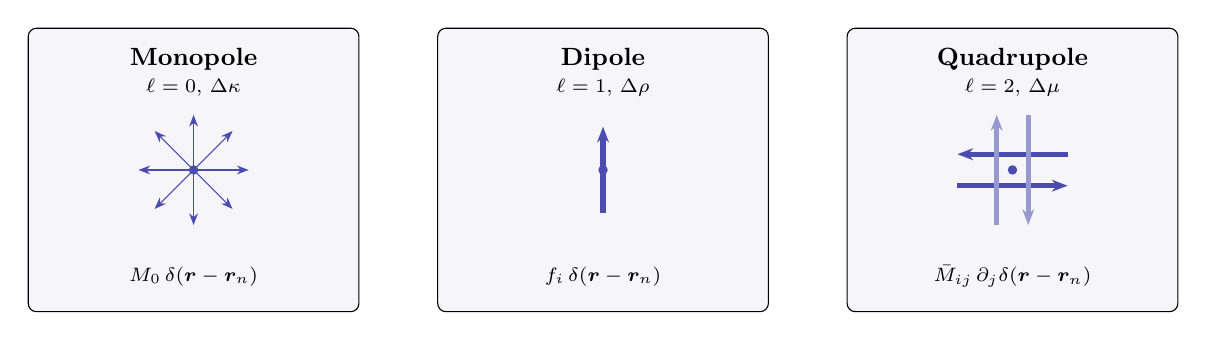
\begin{tikzpicture}[
  every node/.style={font=\small},
  srcbox/.style={draw, rounded corners=3pt, minimum width=42mm, minimum height=36mm, fill=DarkBlue!4},
]
  % Monopole
  \node[srcbox] (mbox) at (0,0) {};
  \node at (0,1.4) {\textbf{Monopole}};
  \node at (0,1.05) {\scriptsize $\ell=0$, $\Delta\kappa$};
  \foreach \a in {0,45,...,315}{
    \draw[-{Stealth[length=1.5mm]}, DarkBlue!70] (0,0) -- (\a:7mm);
  }
  \fill[DarkBlue!70] (0,0) circle (0.6mm);
  \node at (0,-1.35) {\scriptsize $M_0\,\delta(\bm{r}-\rrn)$};

  % Dipole
  \node[srcbox] (dbox) at (5.2,0) {};
  \node at (5.2,1.4) {\textbf{Dipole}};
  \node at (5.2,1.05) {\scriptsize $\ell=1$, $\Delta\rho$};
  \draw[-{Stealth[length=2mm]}, line width=0.7mm, DarkBlue!70]
     (5.2,-0.55) -- (5.2,0.55);
  \fill[DarkBlue!70] (5.2,0) circle (0.6mm);
  \node at (5.2,-1.35) {\scriptsize $f_i\,\delta(\bm{r}-\rrn)$};

  % Quadrupole (double couple)
  \node[srcbox] (qbox) at (10.4,0) {};
  \node at (10.4,1.4) {\textbf{Quadrupole}};
  \node at (10.4,1.05) {\scriptsize $\ell=2$, $\Delta\mu$};
  \draw[-{Stealth[length=2mm]}, line width=0.6mm, DarkBlue!70]
     (10.4-0.7,-0.2) -- (10.4+0.7,-0.2);
  \draw[-{Stealth[length=2mm]}, line width=0.6mm, DarkBlue!70]
     (10.4+0.7,0.2)  -- (10.4-0.7,0.2);
  \draw[-{Stealth[length=2mm]}, line width=0.6mm, DarkBlue!40]
     (10.4-0.2,-0.7) -- (10.4-0.2,0.7);
  \draw[-{Stealth[length=2mm]}, line width=0.6mm, DarkBlue!40]
     (10.4+0.2,0.7)  -- (10.4+0.2,-0.7);
  \fill[DarkBlue!70] (10.4,0) circle (0.6mm);
  \node at (10.4,-1.35) {\scriptsize $\bar{M}_{ij}\,\partial_j\delta(\bm{r}-\rrn)$};
\end{tikzpicture}
\caption{The three effective point sources induced by a small elastic
inclusion.  An isotropic bulk-modulus contrast $\Delta\kappa$ produces a
radial monopole (explosion); a density contrast $\Delta\rho$ produces a
directed dipole aligned with the local displacement; a shear-modulus
contrast $\Delta\mu$ produces a symmetric-traceless quadrupole
(a ``double couple''), shown here as two opposed force pairs whose net
force and net moment both vanish.}
\label{fig:threesources}
\end{figure}

\subsection{How the source writes onto the dependent components}

The link back to the jump conditions of Section~\ref{sec:jumps} is now
transparent.  At leading order the radiation from the
source~\eqref{eq:multipole-final} acts, on a horizontal interface
coinciding with the scatterer layer, exactly as the discontinuity
pattern of Proposition~\ref{prop:dependent}:
\begin{itemize}[leftmargin=1.4em]
  \item The \emph{bulk-modulus} contribution, proportional to
  $M_0 = \Delta\kappa V\,\eps_{kk}$, sources a jump in $\eps_{zz}$ via
  the first term of~\eqref{eq:jump-ezz}.  In the $(\lambda,\mu)$
  parameterisation one has
  $\jump{\lambda}$ and $\jump{\lambda+2\mu}$ acting on $\eps_{kk}$ and
  $\eps_{zz}$ respectively; in the $(\kappa,\mu)$ parameterisation the
  trace part is purely a $\Delta\kappa$ effect.  This is the
  \emph{monopole channel}.
  \item The \emph{shear-modulus} contribution, proportional to
  $\bar{M}_{ij}=2\Delta\mu V\,\eps_{ij}^{\dev}$, sources both a residual
  jump in $\eps_{zz}$ (via the deviatoric part of
  $\jump{\lambda+2\mu}=\jump{\lambda}+2\jump{\mu}$) \emph{and} the
  jumps of $\eps_{xz},\eps_{yz}$ in~\eqref{eq:jump-eaz}.  This is the
  \emph{quadrupole channel}, which spreads across all three dependent
  components.
  \item The \emph{density} contribution, proportional to
  $f_i=\omega^2\Delta\rho V u_i$, does \emph{not} appear in the
  instantaneous jump relations at all: it enters the dynamic balance
  through the inertia term $\rho\omega^2 u_i$ in~\eqref{eq:momentum}
  and is therefore invisible at fixed $\omega$ as a kinematic strain
  discontinuity.  This is the \emph{dipole channel}, which writes onto
  $\uu$ directly rather than onto the strain components.
\end{itemize}

The asymmetry is physically important: \emph{the monopole and
quadrupole channels leave visible signatures on the three dependent
strain components, while the dipole channel acts via the (continuous)
displacement field itself}.  This is precisely why the nine-component
basis~\eqref{eq:psi-nine} is needed: dropping the strain block would
blind the scattering operator to the $\Delta\kappa$ and $\Delta\mu$
channels, and dropping the displacement block would blind it to the
$\Delta\rho$ channel.

%=============================================================================
\section{Block Structure of the Local \emph{T}-Matrix}\label{sec:tblock}
%=============================================================================
The local scattering operator at a single inclusion acts on
$\psi(\rrn)\in\mathbb{C}^9$ as a $9\times 9$ matrix,
\begin{equation}
  T_{\text{loc}}
  \;=\;
  \begin{pmatrix}
    T^{uu} & T^{u\eps}\\[2pt]
    T^{\eps u} & T^{\eps\eps}
  \end{pmatrix},
  \qquad
  T^{uu}\in\mathbb{C}^{3\times 3},\
  T^{\eps\eps}\in\mathbb{C}^{6\times 6},
  \label{eq:T-block}
\end{equation}
with off-diagonal blocks coupling the displacement $\uu$ sector
($\ell=1$, parity-odd) to the strain $\bm{\eps}$ sector
($\ell=0\oplus\ell=2$, parity-even).

\begin{lemma}[Parity selection]\label{lem:parity}
For a centrosymmetric inclusion (i.e.\ one invariant under
$\bm{r}\mapsto -\bm{r}$ about its centre), the Born-level local
operator satisfies
\begin{equation}
  T^{u\eps} \;=\; 0,
  \qquad
  T^{\eps u} \;=\; 0,
  \qquad\text{at leading order in }(ka)^2,
\end{equation}
so that $T_{\text{loc}}$ is block-diagonal between the
$\ell=1$ and $\ell=0\oplus\ell=2$ sectors.
\end{lemma}

\begin{proof}[Sketch]
Under spatial inversion $\bm{r}\mapsto-\bm{r}$, the displacement
$\uu$ is parity-odd (a vector), while the strain tensor $\eps_{ij}$ is
parity-even (a symmetric rank-two tensor on position derivatives).
The Born source density~\eqref{eq:born-source} is therefore parity-odd
in its $\Delta\rho$ term (which acts on $\uu$) and parity-even in its
$\Delta\lambda$ and $\Delta\mu$ terms (which act on $\eps_{ij}$).
Integrating the induced radiation against the centrosymmetric
indicator $\chi_V$ annihilates all parity-mismatched contributions:
a parity-odd source cannot radiate a parity-even response at leading
order through a parity-even geometry, and vice versa.  Hence the
off-diagonal blocks $T^{u\eps}$ and $T^{\eps u}$ vanish at
$O((ka)^2)$.  Sub-leading corrections appear at $O((ka)^4)$ and are
dropped in the long-wavelength limit.
\end{proof}

\begin{proposition}[Block-diagonal structure]\label{prop:blockdiag}
For a centrosymmetric inclusion in the long-wavelength limit, the
local $T$-matrix~\eqref{eq:T-block} reduces to
\begin{equation}
  T_{\text{loc}}
  \;=\;
  \begin{pmatrix}
    T^{uu} & 0\\
    0      & T^{\eps\eps}
  \end{pmatrix},
\end{equation}
with $T^{uu}\propto\Delta\rho\,\omega^2 V\,\mathbb{I}_{3}$ carrying the
dipole (body-force) channel and
$T^{\eps\eps}$ further block-diagonal on the
$(\ell=0)\oplus(\ell=2)$ split of the strain,
\begin{equation}
  T^{\eps\eps}
  \;=\;
  \begin{pmatrix}
    T^{\eps\eps}_{\ell=0} & 0\\
    0 & T^{\eps\eps}_{\ell=2}
  \end{pmatrix},
\end{equation}
with $T^{\eps\eps}_{\ell=0}\propto\Delta\kappa V$ the monopole
(explosion) channel and
$T^{\eps\eps}_{\ell=2}\propto\Delta\mu V$ the quadrupole
(double-couple) channel acting on the five-dimensional deviatoric
subspace.
\end{proposition}

\begin{proof}
By Lemma~\ref{lem:parity} the displacement and strain blocks decouple.
The displacement block carries only the $\Delta\rho$ inertia term
from~\eqref{eq:born-source}, which is a scalar multiple of the
$3\times 3$ identity, giving $T^{uu}\propto\Delta\rho\omega^2 V$.
The strain block carries the two stress contributions from the second
line of~\eqref{eq:born-source}; splitting
the moment tensor as in~\eqref{eq:moment-split} yields a scalar
$M_0=\Delta\kappa V\,\eps_{kk}$ coupled to the trace
$\eps_{kk}$ (the $\ell=0$ channel) and a symmetric traceless
$\bar{M}_{ij}=2\Delta\mu V\,\eps_{ij}^{\dev}$ coupled to the deviator
$\eps_{ij}^{\dev}$ (the $\ell=2$ channel).
By Schur's lemma these two irreducible sectors cannot mix, so
$T^{\eps\eps}$ is itself block-diagonal along the $1+5$ split.
\end{proof}

\begin{remark}[Empirical corroboration]
In the accompanying numerical solver
(\texttt{GlobalMatrix/dressed\_tmatrix.py}) the Born $T$-matrix for a
single cubic inclusion in a homogeneous background is indeed observed
to be block-diagonal in the displacement/strain split to working
precision, with off-diagonal residuals at the level of the $O((ka)^4)$
dispersion correction, consistent with Lemma~\ref{lem:parity}.
\end{remark}

%=============================================================================
\section{Minimality of the Nine-Component Basis}\label{sec:minimality}
%=============================================================================
\begin{theorem}[Minimality]\label{thm:minimal}
Let $T_{\text{loc}}$ be the local scattering operator of a small
isotropic inclusion characterised by three independent Lam\'e
contrasts $(\Delta\lambda,\Delta\mu,\Delta\rho)$, acting in the Born
approximation on the nine-component field
$\psi=(u_i,\eps_{jk})^\top$.  Then the basis~\eqref{eq:psi-nine} is
minimal in the following sense:
\begin{enumerate}[label=(\roman*)]
  \item $T_{\text{loc}}$ has rank $1+1+5=7$: three scalar Lam\'e
  contrasts excite the one-dimensional monopole ($\ell=0$) channel,
  the one-dimensional scalar-on-dipole ($\ell=1$) channel with
  multiplicity $3$ acting as a scalar (so rank~$1$ in the coupling),
  and the five-dimensional quadrupole ($\ell=2$) channel.
  \item No subspace of dimension less than $9$ supports all three
  channels simultaneously: the monopole channel lives in the trace of
  the strain, the dipole channel lives in the displacement, and the
  quadrupole channel lives in the deviator of the strain, and these
  three $\mathrm{SO}(3)$ irreducibles are pairwise orthogonal in
  $\mathbb{C}^9$.
\end{enumerate}
\end{theorem}

\begin{proof}
\textbf{(i).}  In the long-wavelength limit the effective source
density~\eqref{eq:multipole-final} is fully determined by the three
scalars $M_0$, $|f_i|$, and the five independent components of
$\bar{M}_{ij}$, giving a total response rank $1+3+5 = 9$, but the
coupling to the three Lam\'e contrasts reduces the \emph{effective}
rank as follows.  The dipole strength
$f_i=\omega^2\Delta\rho V\, u_i$ couples the three-dimensional
displacement subspace to itself via a scalar $\Delta\rho$, so the
corresponding $T^{uu}$ block is a multiple of the identity and has
effective source-side rank $1$ (it adds the same contrast to all three
components).  The monopole $M_0=\Delta\kappa V\,\eps_{kk}$ couples the
one-dimensional trace subspace to itself with scalar $\Delta\kappa$,
contributing rank $1$.  The quadrupole
$\bar{M}_{ij}=2\Delta\mu V\,\eps_{ij}^{\dev}$ couples the
five-dimensional deviator subspace to itself with scalar
$\Delta\mu$, so $T^{\eps\eps}_{\ell=2}$ is a multiple of the identity
on $\mathbb{R}^5$ and contributes rank $5$.  Total
$1+1+5=7$.

\textbf{(ii).}  Suppose $V'\subset\mathbb{C}^9$ is a subspace of
dimension $d<9$ that supports all three channels.  By
$\mathrm{SO}(3)$ invariance the projection onto each irreducible
sector must be either zero or full-rank on that sector.  The monopole
sector has dimension $1$, the dipole $3$, and the quadrupole $5$.  If
all three projections are full-rank, then $V'$ contains the direct
sum $1\oplus 3\oplus 5 = \mathbb{C}^9$, so $d=9$, a contradiction.
Hence at least one sector is absent, and the corresponding Lam\'e
contrast cannot be represented.
\end{proof}

\begin{remark}
Theorem~\ref{thm:minimal} is the reason the solver in
\texttt{GlobalMatrix/block\_riccati\_cluster.py} uses a $9\times 9$
$T$-matrix rather than the smaller $3\times 3$ (displacement-only)
or $6\times 6$ (strain-only) options: both of the latter two would
silently discard one of the three Lam\'e-contrast channels and yield a
quantitatively wrong Foldy-Lax solution.  A $4\times 4$ ``acoustic''
basis carrying $(p,\bm{v})$ recovers only the monopole and dipole
channels and misses the quadrupole entirely.
\end{remark}

%=============================================================================
\section{Conclusions}\label{sec:conclusions}
%=============================================================================
The three effective multipole sources emitted by a small elastic
inclusion are in one-to-one correspondence with the three independent
Lam\'e contrasts and with the three $\mathrm{SO}(3)$ irreducible
components of the nine-dimensional displacement-strain state vector.
Specifically, the monopole channel ($\ell=0$, driven by
$\Delta\kappa$) lives in the trace of the strain; the dipole channel
($\ell=1$, driven by $\Delta\rho$) lives in the displacement; and the
quadrupole channel ($\ell=2$, driven by $\Delta\mu$) lives in the
deviator of the strain.  The three strain components carrying a
normal derivative across a horizontal interface --- $\eps_{zz}$,
$\eps_{xz}$ and $\eps_{yz}$ --- are the \emph{dependent} components,
and they are exactly those on which the monopole and quadrupole
channels write their signatures via the closed-form jump relations
\eqref{eq:jump-ezz}--\eqref{eq:jump-eaz}.  The dipole channel does not
appear in the kinematic strain jumps at all but instead acts
dynamically via the continuous displacement field.  An elementary
parity argument, sharpened by Schur's lemma, gives the local
$T$-matrix a block-diagonal structure that reflects this
decomposition, and the nine-component basis is minimal in the sense
that no smaller subspace can carry all three Lam\'e-contrast channels
simultaneously.

This structural understanding underpins the block-preconditioned
Foldy-Lax solver of the companion
paper~\cite{nestor2026blockfoldylax}: the $9\times 9$ basis is
\emph{necessary} to capture the full physics, the block-diagonal
$T$-matrix structure justifies caching the local scattering operator
by contrast channel, and the parity-based selection rules can be
exploited in a future optimisation to reduce the arithmetic of the
$2$D FFT convolution from nine to the three independent sector sizes
$1$, $3$ and $5$.

\begin{thebibliography}{9}

\bibitem{foldy1945}
L.L.~Foldy,
\emph{The multiple scattering of waves.  I.  General theory of isotropic
scattering by randomly distributed scatterers},
Phys.\ Rev.\ \textbf{67}, 107--119 (1945).

\bibitem{lax1951}
M.~Lax,
\emph{Multiple scattering of waves},
Rev.\ Mod.\ Phys.\ \textbf{23}, 287--310 (1951).

\bibitem{backus1976}
G.~Backus and M.~Mulcahy,
\emph{Moment tensors and other phenomenological descriptions of seismic
sources --- I.\ Continuous displacements},
Geophys.\ J.\ R.\ astr.\ Soc.\ \textbf{46}, 341--361 (1976).

\bibitem{akirichards2002}
K.~Aki and P.G.~Richards,
\emph{Quantitative Seismology}, 2nd edition,
University Science Books, Sausalito, CA (2002).

\bibitem{kennett2001}
B.L.N.~Kennett,
\emph{The Seismic Wavefield, Volume I: Introduction and Theoretical
Development},
Cambridge University Press (2001).

\bibitem{martin2006}
P.A.~Martin,
\emph{Multiple Scattering: Interaction of Time-Harmonic Waves with
$N$ Obstacles},
Cambridge University Press (2006).

\bibitem{nestor2026blockfoldylax}
T.M.~Nestor,
\emph{Block-Preconditioned Foldy-Lax Solver for Layered Elastic Media},
Companion paper, SeismicInversion repository (2026).

\bibitem{nestor1996phd}
T.M.~Nestor,
\emph{Multiple scattering of elastic waves in layered media with
space-filling heterogeneities},
Ph.D.\ thesis, University of Cambridge (1996).

\end{thebibliography}

\end{document}

